\section{Mission Overview}

\subsection{Mission Definition}
The Cluster-II Mission is planned and executed by the European Space Agency and was launched on 16th of July 2016. The whole mission consists of four identical spacecrafts flying in a tetrahedral formation in a highly elliptical orbit, where each spacecraft is collecting various data on the space environment with its 11 scientific payload instruments. These in-situ measurements are done to build a very accurate 3D-Model of the earth's magnetosphere and thus to observe the magnetosphere interaction with the solar wind not only in a spatial but also in a temporal resolution.

The main goal of this mission is to examine and gather data especially on the plasma structures in the bow shock region, the magnetopause, polar cusps, the earth's magnetotail and the auroral zone, all of them regions with very interesting properties when it comes to the interaction with solar wind \citep{ESA:clusterWebsite}.

\begin{figure}[h]
	\centering
	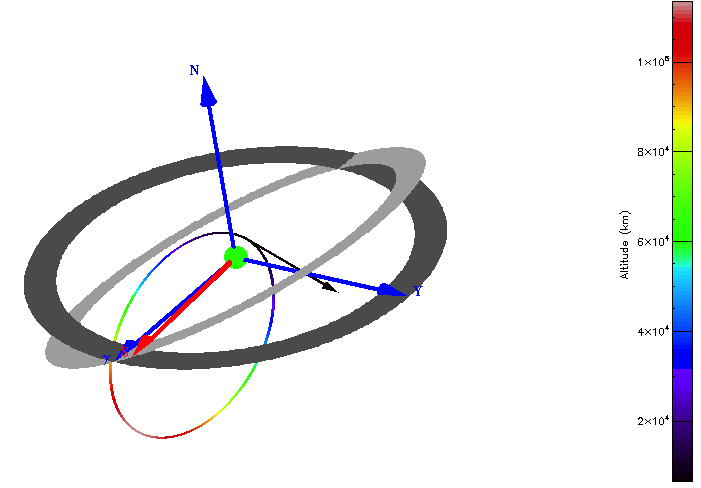
\includegraphics[width=\linewidth]{spenvis/3d_gei}
		\caption{One Orbit of FM-8 Tango, the color bar shows the altitude}
	\label{fig:orbit}
\end{figure}
To model the Orbit of FM-8 Tango a set of TLE (Two Line Element) data provided by CelesTrak was used \citep{celesTrak}.\\
Figure \ref{fig:orbit} shows one orbit of FM-8 Tango and indicates the altitude of the orbit. The orbit itself is a retrograde orbit with an inclination of 131.6 degrees. A complete set of TLE data describing all important orbit parameters can be found in the Appendix \ref{tleParameters}.




\subsection{Space Environment}

\subsection{Radiation Environment}

